
% {{{ preamble

\documentclass{article}

\usepackage{url}
\usepackage{hyperref}
\usepackage{graphicx}
\usepackage{tikz}
\usepackage{tikz-timing}
\usepackage{nonfloat}
\usepackage{amsmath}
\usepackage{mathtools}
\usepackage{fancyvrb}
\usepackage{parskip}

\usepackage{courier}
\usepackage{listings}
\lstset{numbers=left,
		language=C,
		tabsize=4,
		basicstyle=\ttfamily,
		%basicstyle=\footnotesize,
		showstringspaces=false,  % don't show the space character
		%commentstyle=\textit,
		showtabs=false,
		extendedchars=true,
		basicstyle=\normalsize,
		captionpos=b,
		frame=tb,
		xleftmargin=0.3in}

\usepackage{vmargin}  % make the margins a bit smaller
%\setmarginsrb{1.0in}{1.0in}{1.0in}{1.0in}{0in}{0.4in}{0.0in}{0.40in}
\setmarginsrb{1.0in}{1.0in}{1.0in}{1.0in}{0in}{0.25in}{0in}{0.20in}

\raggedright

\usepackage[backend=biber,autocite=footnote,
			bibstyle=authortitle,citestyle=verbose-inote]{biblatex}
\setlength{\bibitemsep}{\baselineskip}

\addbibresource{references.bib}

% }}}

\begin{document}

\VerbatimFootnotes

% {{{ title page

\thispagestyle{empty}

\centerline{\Large \textbf{Learning Linux Device Drivers}}
\vspace{0.1in}
\centerline{\normalsize {Jeremiah Mahler} ({\href{mailto:jmmahler@gmail.com}{jmmahler@gmail.com}})}
\centerline{\small \today}
\vspace{0.2in}

% }}}

\tableofcontents
\pagebreak

% {{{ Introduction
\section{Introduction}

\begin{figure*}[h!]
\begin{center}
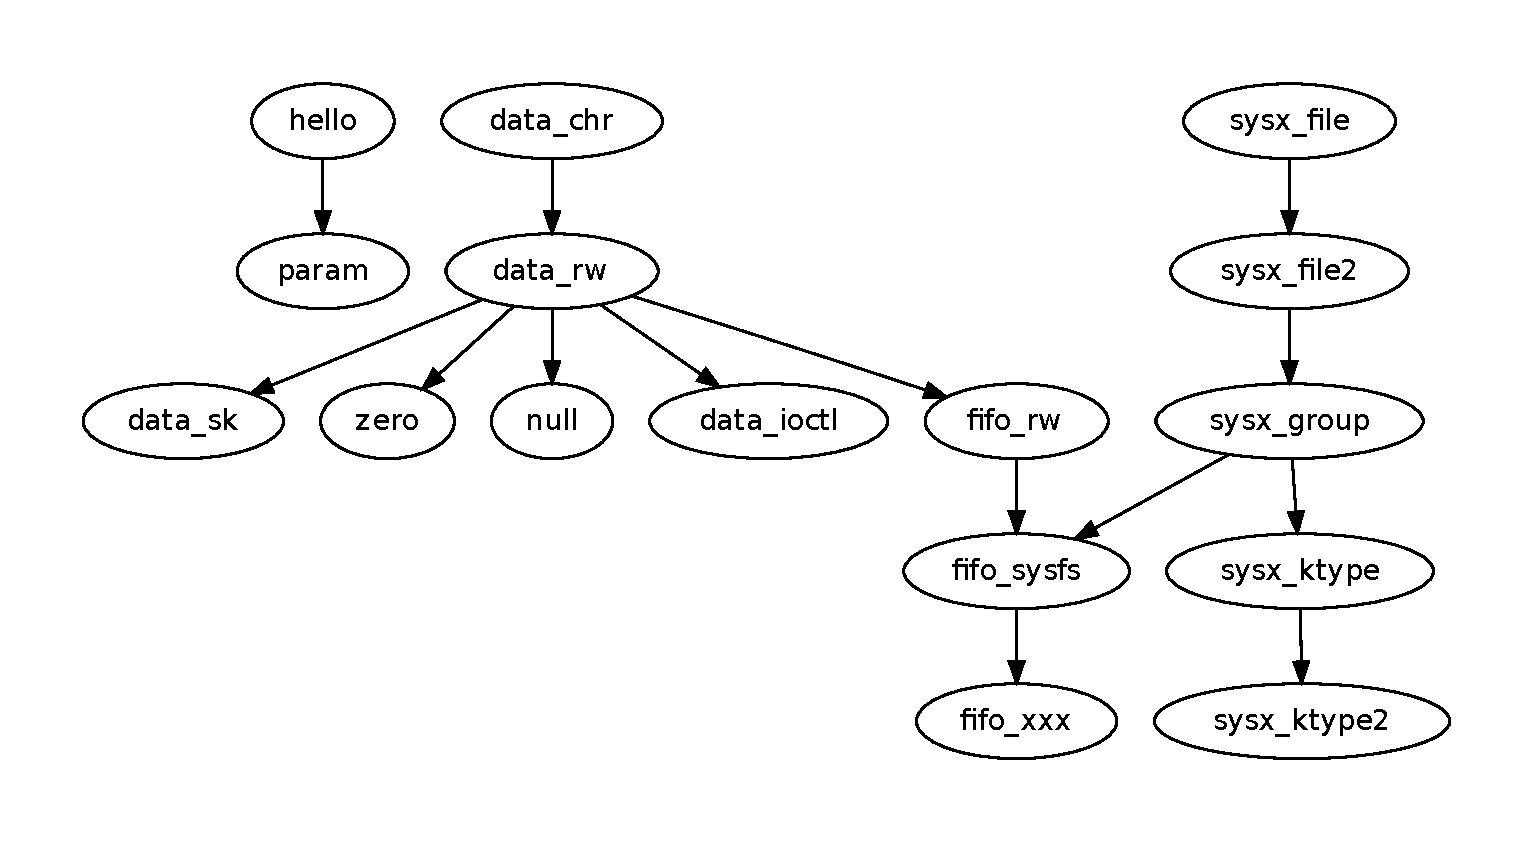
\includegraphics[scale=0.6]{hierarchy/hier}
\end{center}
\caption{Hierarchy of kernel module examples.  Simplest at the
top downward to the more complex.}\label{fig:hier}
\end{figure*}

There are many excellent books about Linux device drivers
\autocite{corbet2009linux}
\autocite{venkateswaran2008essential}
\autocite{love2010linux}
\autocite{love2013linux}.
However, in this authors experience, they were difficult to learn from.
It certainly was not from their lack of detail.
Clearly each of the authors have a profound understanding of the Linux
kernel and their books reflect this.
If anything it is due to this lack of simplicity.

The drivers described in this document aim to be simple and concise.
Each one introduces as few concepts as possible.
And each driver is a fully working example
\footnote{Be creative with the examples.
Try changing something and see what happens.
Actively exploring in this way is a great way to solidify your understanding.}.
Many of the drivers are built in stages.
Each stage introduces a new concept.
And the changes are concisely described showing the
differences (\verb+diff+).
Figure \ref{fig:hier} shows the hierarchy of driver examples.

% }}}

\section{Hello, World}

% {{{ hello
\subsection{hello}

The \verb+hello+ module (Listing \ref{lst:hello}) simply prints message
when it is loaded and unload.

\begin{verbatim}
hello$ make
 (should compile without error, resulting in hello.ko)
hello$ sudo insmod hello.ko
 Hello, World
hello$ sudo rmmod hello
 Goodbye, cruel world
\end{verbatim}

\lstinputlisting[float=ht,
				 caption={Hello, World module in hello/hello.c},
			 	 label={lst:hello}]
	{../hello/hello.c}

The \verb+module_init+ (line 18) and \verb+module_exit+ (line 19) tell
the kernel which functions to call when this module is
loaded (\verb+insmod+) and unloaded (\verb+rmmod+).

The \verb+__init+ (line 4) and \verb+__exit+ (line 10)
are optional hints for the compiler.  For example in the case of
\verb+__init+, this tells the kernel that it may discard the code
after initialization has been completed.

Both the init function (line 4) and the exit function (line 10)
are declared \verb+static+.
Since these functions are not meant to be used outside the scope
of this file, declaring them \verb+static+ enforces this
constraint\autocite[Pg. 52]{corbet2009linux}.

The \verb+printk+ statements are the \verb+printf+ of the
kernel domain.  There are various levels, in this case
\verb+KERN_ALERT+ is used which will cause the messages
to appear on the console.  Notice that there is no comma
between the level and the message.

The \verb+MODULE_AUTHOR+ and \verb+MODULE_LICENSE+ on lines 15 and 16
are optional but recommended\autocite[Pg. 51]{corbet2009linux}.
There are various other \verb+MODULE_*+
options as well (\verb+linux/module.h+).
% }}}

% {{{ param
\clearpage
\subsection{param}

The \verb+param+ module expands upon the \verb+hello+ module to
take a parameter specifying how many times to print the message.

\begin{verbatim}
param$ sudo insmod hello.ko howmany=2
 Hello, World
 Hello, World
param$ sudo rmmod hello
 Goodbye, cruel world
 Goodbye, cruel world
\end{verbatim}

Listing \ref{lst:param-diff} shows the differences between this
parameterized hello world module and the previous \verb+hello+ module.

\lstinputlisting[float=ht,
				 caption={param\$ diff -u hello.c ../hello/hello.c},
			 	 label={lst:param-diff}]
	{../param/diff}

To use a parameter a global variable has been created named \verb+howmany+
on line 8.
And on line 9 the \verb+module_param+ function is used to tell
the kernel about this parameter
\footnote{The \verb+module_param+ function create a sysfs entry
in \verb+/sys/module/parameters/howmany+.  \verb+sysfs+ will
be discussed in detail in later modules.}.

On lines 13-19 and 25-30 it can be seen that the same message
is printed \verb+howmany+ times.
% }}}

\section{Character Devices}

The \verb+data+ module allocates some memory which can
then be read from and written to.
This is accomplished as a character device and supports all
the usual file operations.

% {{{ data_chr
\subsection{data\_chr}
\label{sec:data_chr}

The first step is to construct the basic infrastructure for
a character driver as shown in Listing \ref{lst:data_chr}.
It doesn't do anything useful but it will simplify the description
of upcoming drivers.

The \verb+DEVICE_NAME+ (line 8) is just a shortcut for the
name which is used in several places.

Lines 10-17 are the global variables that will be used.
The \verb+struct data_dev+ is the per device structure.
Notice that a character device is placed inside.

The \verb+file_operations+ (line 19-21) in this case only
defines the \verb+.owner+.  Upcoming modules will add references
to the open, close, read, write, and seek functions to this structure.

\verb+alloc_chrdev_region+ (line 26) allocates a major and minor number
for the character device\autocite[Pg. 66]{corbet2009linux}.
In this case only one major and minor pair is needed.

Functions such as \verb+alloc_chrdev_region+ may fail and when they
do anything that has been created up to that point must be undone
to ensure the kernel is left in a consistent state.
A common way this is done is using \verb+goto+ statements which
branch to different steps in the exit
sequence\autocite[Pg. 53]{corbet2009linux}.
It can be seen that if \verb+alloc_chrdev_region+ fails its \verb+goto+
(line 29) will branch to line 66.
Since nothing was created up to that point nothing has to be undone.

\verb+class_create+ (line 32) establishes a ``class'' for this
module which is also represented in sysfs under \verb+/sys/class/data+.
This object will be used later as an argument to \verb+device_create+.

Since the per device structure is just a pointer it must be
allocated before it is used (line 32).

To establish the character device it must be initialized and
added (lines 41-43).  And finally the device is created (line 49).
This device will now appear under \verb+/dev/data0+.

\pagebreak
\lstinputlisting[caption={data\_chr driver.},
			 	 label={lst:data_chr}]
	{../data_chr/data.c}


% }}}

% {{{ data_rw
\clearpage
\subsection{data\_rw}
\label{sec:data_rw}

With the addition of read/write operations the device can be
operated upon just like any other file.
As an example the driver source code can be copied in to the
device and then read back out.
The result should be the same up to the maximum amount which
in this case was 128 bytes.
This maximum size is a \verb+#define+ inside the driver.

\begin{verbatim}
$ sudo dd if=data.c of=/dev/data0 bs=128 count=1

$ sudo dd if=/dev/data0 of=output bs=128 count=1
\end{verbatim}

Listing \ref{lst:data_rw-diff} shows the differences compared to the
previous \verb+data_chr+ driver.  An array of bytes has been added
to the per device structure along with the current offset (lines 7-17).

File operations for open, read, write and release have been added (lines 82-88).
The release operation is called when a process closes the device file.

When the file is opened the open function (lines 19-29) is called.
The \verb+container_of+ function (line 23) is used to obtain a parent
structure from a child structure\autocite[Pg. 79]{corbet2009linux}
\autocite{kroah2005cont}.
Recall that the per device structure, \verb+data_devp+ contains a
\verb+cdev+ (line 14).
\verb+container_of+ makes it possible to obtain the \verb+data_devp+
from the \verb+cdev+.

The open functions sets the offset to zero (line 24) when is the usual
behavior when opening a file.

The open function also stores the device structure under \verb+private_data+
(line 26) so it is easy to access in the read/write functions.

When data is read from the device file the read function (lines 31-52)
is called.
Since the amount of data that can be read is limited by \verb+MAX_DATA+
the amount requested will be reduced it it is too large (lines 39-43).
Then the \verb+copy_to_user+ function is used to attempt to transfer
the data in to user space (lines 45-47).
The \verb+copy_to_user+ also hecks to make sure that destination it is
transferring to is valid for the given process.
If the transfer was a success the new offset is stored (line 49)
and then the number of bytes that were successfully transfered are
returned (line 51).

The write function (lines 54-70) has the same operation as read
except in the opposite directory.
Notice that the \verb+copy_from_user+ (line 68) function is used
in this case.

And since nothing needs to be done when the device is closed,
the release function (lines 77-80) simply returns success.

\pagebreak
\lstinputlisting[caption={data\_rw\$ diff -u ../data\_chr/data.c data.c},
			 	 label={lst:data_rw-diff}]
	{../data_rw/diff}

% }}}

% {{{ data_sk
\clearpage
\subsection{data\_sk}

To add support for the seek operation requires the addition of
one more function along with its corresponding entry in the
file operations.  Listing \ref{lst:data_sk-diff} shows the
differences.

\lstinputlisting[caption={data\_sk\$ diff -u ../data\_rw/data.c data.c},
			 	 label={lst:data_sk-diff}]
	{../data_sk/diff}

To test the seek operations a seek-able cat program named \verb+cats+
has been created.

\begin{verbatim}
jeri@crowe:~/ldd/data_sk/test$ sudo wc -c /dev/data0
128 /dev/data0
jeri@crowe:~/ldd/data_sk/test$ sudo dd if=cats.c of=/dev/data0 bs=128 count=1
jeri@crowe:~/ldd/data_sk/test$ sudo ./cats /dev/data0 END -28
t the reset of 'file.txt'
 *jeri@crowe:~/ldd/data_sk/test$ 
jeri@crowe:~/ldd/data_sk/test$ sudo ./cats /dev/data0 SET 100
t the reset of 'file.txt'
 *jeri@crowe:~/ldd/data_sk/test$ exit
\end{verbatim}

Notice that the file is 128 bytes total.
The output after seeking from the start forward 100 bytes produces
the same result as seeking backward 28 bytes from the end.
In this instance the device is operating correctly.

% }}}

% {{{ data_ioctl
\subsection{data\_ioctl}

Using \verb+ioctl()+ for new designs is not recommended\autocite[Pg. 156]{corbet2009linux}\autocite{love2010linux}.
Instead \verb+sysfs+ is preferred.
While \verb+/proc+ is another option, it is also becoming obsolete in
favor of \verb+sysfs+.
Nonetheless it is still used so it is worth knowing how it works.

Include with this driver is a test program (\verb+data_ioctl/test/ioctlx.c+).
The driver allows the reset, read and write of a single global variable
(\verb+x+) in the driver.
The test program allows these operations to be performed.

\begin{verbatim}
data_ioctl$ cd test/
test$ sudo ./ioctlx 10    # set value
test$ sudo ./ioctlx       # read current value
 10
test$ sudo ./ioctlx 0     # reset
test$ sudo ./ioctlx
 0
test$
\end{verbatim}

The \verb+data_ioctl+ driver has the fewest number of differences compared to
the \verb+data_chr+ driver (Section \ref{sec:data_chr}) as shown
in Listing \ref{lst:data_ioctl-diff}.
The open (lines 10-19) and release (lines 75-78) are the same as
those for the \verb+data_rw+ driver (Section \ref{sec:data_rw}).
The only code of interest is for the \verb+data_ioctl+ function (lines 29-73).

The first thing to notice is the use of "magic" (lines 23-25, 37).
Magic is used to make the ioctl calls unique across the entire system
which helps prevent inadvertent configuration if the wrong device is opened
\autocite[Pg. 158]{corbet2009linux}.
The user program must also contain the corresponding magic
values as is done in the test program (Listing \ref{lst:data_ioctl-magic}).

The three defines (lines 23-24) describe the supported ioctl operations.
Any number of additional operations can be added.
And it can be seen that there is an operation that has no data (\verb+_IO+),
reads data (\verb+_IOR+) and writes data (\verb+_IOW+).
The \verb+DATA_IOC_MAXNR+ (line 27) is used as a sanity check later (line 41).

And the switch statement (lines 53-70) process the ioctl commands.
In this case all the operations involve the global variable \verb+x+.
It is either reset, read or written.

\pagebreak
\lstinputlisting[caption={data\_ioctl\$ diff -u ../data\_chr/data.c data.c},
			 	 label={lst:data_ioctl-diff}]
	{../data_ioctl/diff}

\lstinputlisting[linerange=9-19,
				firstnumber=9,
				caption={Corresponding "magic" in user program.},
				label={lst:data_ioctl-magic}]
	{../data_ioctl/test/ioctlx.c}

% }}}

% {{{ null, zero
\subsection{null, zero}

From what has been described so far it is easy construct a driver
for the well known \verb+/dev/null+ and \verb+/dev/zero+ devices.

The zero device is even simpler than the \verb+data_rw+ example
(Section \ref{sec:data_rw}).
The only real difference, other than names (\verb+data+ -$>$ \verb+null+),
is the read and write operations as shown in Listing \ref{lst:null}.

\lstinputlisting[linerange=30-40,
				firstnumber=30,
				caption={/dev/null read and write functions.},
				label={lst:null}]
	{../null/null.c}

The read and write functions for the \verb+zero+ driver are also quite
simple (Listing \ref{lst:zero}.
The one new addition is the \verb+clear_user+ function.
It behaves like the \verb+copy_to_user+ function except that it simply
zeros out the users buffer.

\lstinputlisting[linerange=30-44,
				firstnumber=30,
				caption={/dev/zero read and write functions.},
				label={lst:zero}]
	{../zero/zero.c}

% }}}

\subsection{fifo\_rw}

\section{Sysfs}
\subsection{sysx\_file}
\subsection{sysx\_file2}
\subsection{sysx\_group}
\subsection{sysx\_ktype}
\subsection{sysx\_ktype2}
\subsection{data\_sysfs}
\subsection{fifo\_sysfs}

\section{Concurrency}
\subsection{data\_xxx}
\subsection{fifo\_xxx}
\subsection{fifo\_fix}

\pagebreak
\printbibliography

%\pagebreak
%\printindex

\end{document}
